\documentclass[tikz]{standalone}
\usepackage{pgfplots}
\pgfplotsset{compat=1.18}
\begin{document}
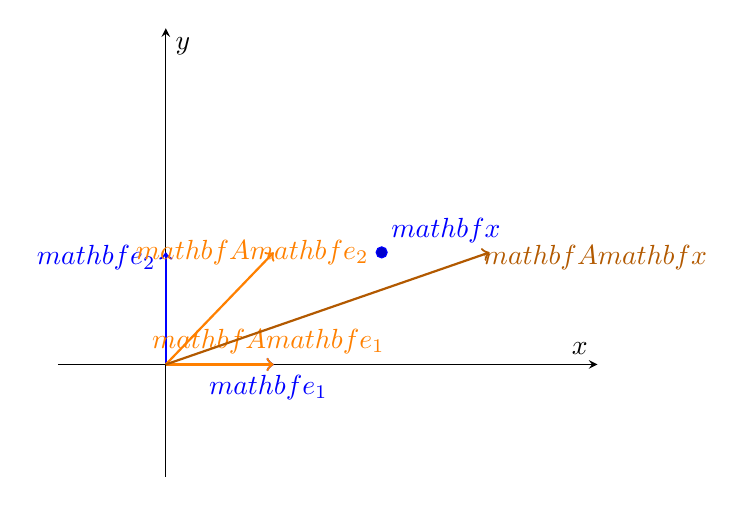
\begin{tikzpicture}
  \begin{axis}[
      axis lines=middle,
      xmin=-1, xmax=4,
      ymin=-1, ymax=3,
      xlabel={$x$}, ylabel={$y$},
      ticks=none, clip=false,
      legend style={at={(0.02,0.98)},anchor=north west}
  ]
    % original basis
    \addplot[->,thick,blue] coordinates {(0,0) (1,0)} node[pos=0.95,below] {$\\mathbf{e}_1$};
    \addplot[->,thick,blue] coordinates {(0,0) (0,1)} node[pos=0.95,left] {$\\mathbf{e}_2$};
    % transformed basis
    \addplot[->,thick,orange] coordinates {(0,0) (1,0)} node[pos=0.95,above] {$\\mathbf{A}\\mathbf{e}_1$};
    \addplot[->,thick,orange] coordinates {(0,0) (1,1)} node[pos=0.8,above] {$\\mathbf{A}\\mathbf{e}_2$};
    % sample point
    \addplot+[only marks,mark=*] coordinates {(2,1)} node[above right] {$\\mathbf{x}$};
    \addplot[->,thick,orange!70!black] coordinates {(0,0) (3,1)} node[pos=0.95,right] {$\\mathbf{A}\\mathbf{x}$};
  \end{axis}
\end{tikzpicture}
\end{document}
